\setcounter{chapter}{8}
\setcounter{section}{0}
\setcounter{figure}{0}
\setcounter{equation}{0}
\setcounter{table}{0}
\chapter*{
\includegraphics[width=\textwidth]{./figures/Topic8/Topic8.jpg}}
\addcontentsline{toc}{chapter}{Topic 8: Statistical Mechanics in Biology}

\section{Introduction}
One goal of systems biology is to integrate information about DNA, RNA, proteins, and all the interactions between them to build a predictive model of how a cell operates.  This involves tracking the interaction between trillions of atoms—how do we deal with it?  
Even today’s most powerful supercomputers cannot handle such a problem.  Instead of attempting to precisely describe the motion of each atom or molecule in a system, it is best to restrict calculations to averaged quantities, or probabilistic outcomes.  A branch of physics called statistical mechanics helps us make simple predictions about the average energy content of an atom or molecule and the probability of its existence in a specific configuration.  
The relationship between energy and probability is at the heart of many theories in modern biophysics.  We will first introduce basic concepts in statistical mechanics before examining how it can be applied to some key concepts, including membrane potentials and protein folding.

\section{Degrees of Freedom}

Degrees of freedom can loosely be thought of as independent ways in which an atom or molecule can move through space.  Since space is described by three independent directions ($x$, $y$, and $z$), an atom has three translational degrees of freedom.  Molecules can also rotate and/or vibrate, allowing other degrees of freedom.  In statistical mechanics, degrees of freedom are defined more rigorously as energies of the form $E(q) = cq^2$, where $q$ is a dynamic variable (e.g. $v_x$, $x$, or $\omega_x$) and $c$ is a constant.  Below are several examples of degrees of freedom:
\begin{align}
E\left(v_x\right) &= \frac{1}{2}mv_x^2 &{\rm Translational}\nonumber\\
E\left(x\right) &= \frac{1}{2}kx^2 &{\rm Vibrational}\nonumber\\
E\left(\omega_x\right) &= \frac{1}{2}I\omega_x^2 &{\rm Rotational}\nonumber
\end{align}

When a system of atoms or molecules is at thermal equilibrium with its environment at a  constant temperature $T$ (measured in Kelvin), one can prove with statistical mechanics that the average energy found in each degree of freedom is always $\frac{1}{2}k_BT$, where the Boltzmann constant $k_B = 1.38\times10^{-23}$ J/K.

\section{Probability and the Boltzmann Factor}

To illustrate the connection between energy and probability, let us consider a simple system of identical atoms capable of sharing identical quanta of energy.  Because every atom in the system continuously exchanges energy with the other atoms, the system can be found in a number of possible energy distributions.  If our system has five atoms and only one quantum of energy to be shared between the atoms, there are five possible ways in which the quantum can be distributed:
\begin{table}[htb]
\begin{center}
\begin{tabular}{ccccc}
\hline
Atom 1 & Atom 2 & Atom 3 & Atom 4 & Atom 5 \\
\hline
1 &	0 &	0 &	0 &	0\\
0 &	1 &	0 &	0 &	0\\
0 &	0 &	1 &	0 &	0\\
0 &	0 &	0 &	1 &	0\\
0 &	0 &	0 &	0 &	1\\
\hline
\end{tabular}
%\caption{Intensity levels in decibels for several common sources of sound.}
\label{table8-1}
\end{center}
\end{table}
The probability $P$ that a given atom has 1 quantum of energy is $P(1) = 1/5 = 0.2$. The probability $P$ that a given atom has 0 quanta of energy is $P(0) = 4/5 = 0.8$.

Now consider the same system of five atoms, but add an extra quantum of energy.  Now there are fifteen ways to distribute the energy:
\begin{table}[htb]
\begin{center}
\begin{tabular}{ccccc}
\hline
Atom 1 & Atom 2 & Atom 3 & Atom 4 & Atom 5 \\
\hline
2 &	0 &	0 &	0 &	0\\
0 &	2 &	0 &	0 &	0\\
0 &	0 &	2 &	0 &	0\\
0 &	0 &	0 &	2 &	0\\
0 &	0 &	0 &	0 &	2\\
1 &	1 &	0 &	0 &	0\\
1 &	0 &	1 &	0 &	0\\
1 &	0 &	0 &	1 &	0\\
1 &	0 &	0 &	0 &	1\\
0 &	1 &	1 &	0 &	0\\
0 &	1 &	0 &	1 &	0\\
0 &	1 &	0 &	0 &	1\\
0 &	0 &	1 &	1 &	0\\
0 &	0 &	1 &	0 &	1\\
0 &	0 &	0 &	1 &	1\\
\hline
\end{tabular}
%\caption{Intensity levels in decibels for several common sources of sound.}
\label{table8-2}
\end{center}
\end{table}
The probability $P$ that a given atom has 2 quanta of energy is $P(2) = 1/15 = 0.067$. The probability $P$ that a given atom has 1 quantum of energy is $P(1) = 4/15 = 0.267$. The probability $P$ that a given atom has 0 quanta of energy is $P(0) = 10/15 = 0.667$.

In the above situation, two quanta distributed among five atoms yields an average energy of 0.4 quanta/atom.  If we keep this average the same but double the number of quanta and the number of atoms (four quanta among ten atoms), the possible number of combinations grows significantly.  With some effort, we can show that:
\begin{align}
P(4) &= 1/715 = 0.00140\nonumber\\
P(3) &= 9/715 = 0.0126\nonumber\\
P(2) &= 45/715 = 0.0629\nonumber\\
P(1) &= 165/715 = 0.231\nonumber\\
P(0) &= 495/715 = 0.692.\nonumber
\end{align}

If we tried to use this method for biological samples with trillions of atoms or molecules per cell, it would take forever, even with the enormous computational power of today’s computers.  It is simply unreasonable to consider all possible combinations in a realistic atomic model of a biological sample.  Fortunately, there is another way.

For large-scale samples, there is an analytical formula that works well in predicting the probability that a system of atoms contains a certain amount of thermal energy.  To appreciate the origin of this formula, consider how the probabilities $P(E)$ in the example discussed above (4 quanta between 10 atoms) vary with the energy $E$. 
\begin{figure}[htb]
	\centering
	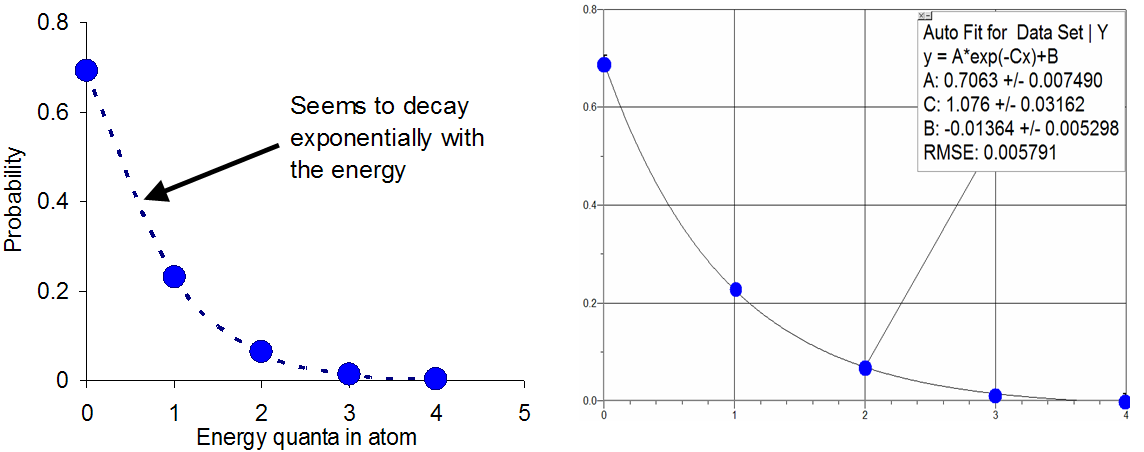
\includegraphics[width=\textwidth]{./figures/Topic8/Fig8-1.png}
	\caption{The graph on the left clearly shows that the probabilities decay with increasing energy in a way hat seems exponential. The graph on the right shows that in fact the points follow a curve fit to such a function.}
 	\label{Fig8-1}
\end{figure}
The tendency for the probabilities to day exponentially is at the heart of what is known as the Boltzmann factor, which predicts that when an atom or molecule is in thermal equilibrium with the others, the probability $P$ of finding the atom with a certain energy $E$ is proportional to
\begin{equation}\label{eqn8-1}
P\left(E\right)\propto{\rm e}^{-E/k_BT}
\end{equation}
Because the constant in front of the exponential term (sometimes referred to as the pre-exponential) is not always easy to find, it is actually more helpful to use the relation Eq.~\ref{eqn8-1} for calculating ratios of probabilities.  For instance, the probability of finding the atom or molecule in state $E_2$ relative to the probability of finding the same atom or molecule in state $E_1$ is
\begin{eqnarray}\label{eqn8-2}
\frac{P\left(E_2\right)}{P\left(E_1\right)} &=& \frac{C{\rm e}^{-E_2/k_BT}}{C{\rm e}^{-E_1/k_BT}}\nonumber\\
&=& \frac{{\rm e}^{-E_2/k_BT}}{{\rm e}^{-E_1/k_BT}}\nonumber\\
&=& {\rm e}^{-\left(E_2-E_1\right)/k_BT}
\end{eqnarray}

To demonstrate that this formula works, let us estimate $P(1)/P(0)$ with the system of four quanta distributed among ten atoms.  The average energy per atom is 0.4 quanta, and each atom has only one degree of freedom.  Since each degree of freedom has an average energy equal to $\frac{1}{2}k_BT$, it is true that $\frac{1}{2}k_BT$ = 0.4 quanta.  Simplifying, $k_BT$ = 0.8 quanta.  According to Eq.~\ref{eqn8-2}, 
\begin{eqnarray}
\frac{P\left(1\right)}{P\left(0\right)} &=& {\rm e}^{-\left(E_2-E_1\right)/k_BT}\nonumber\\
&=&  {\rm e}^{-\left(1-0\right)/0.8}\nonumber\\
&=& 0.29\nonumber
\end{eqnarray}
This ratio of probabilities, which is estimated from the Boltzmann factors, is in fact in good agreement with the ratio of the actual probabilities:
\begin{eqnarray}
\frac{P\left(1\right)}{P\left(0\right)} &=& \frac{165/715}{495/715}\nonumber\\
&=&  \frac{165}{495}\nonumber\\
&=& 0.33\nonumber
\end{eqnarray}
Statistical mechanics shows that the agreement between estimated and actual probability ratios improves as the number of particles and the number of quanta grow.  Thus for biological samples with particles and quanta on the order of Avogadro's number, the Boltzmann factor is well suited to predict probabilistic outcomes.  Some of those applications, including membrane potentials and protein folding are discussed next.  

\section{Applications of Statistical Mechanics}

\subsection{Membrane Potentials}

An important application of the Boltzmann factor in biology is in understanding the relationship between the electric potential across a cell membrane and the concentration of ions on either side of the membrane.  Recall that there is no absolute electric potential; it is always measured relative to something.  Here, we will derive the potential on the outside of the cell relative to the potential on the inside, a quantity that will be expressed in terms of ionic concentration in those two regions.  In Figure \ref{Fig8-2} below, $V_{out}$ is the outside potential and $V_{in}$ is the inside potential.    
\begin{figure}[htb]
	\centering
	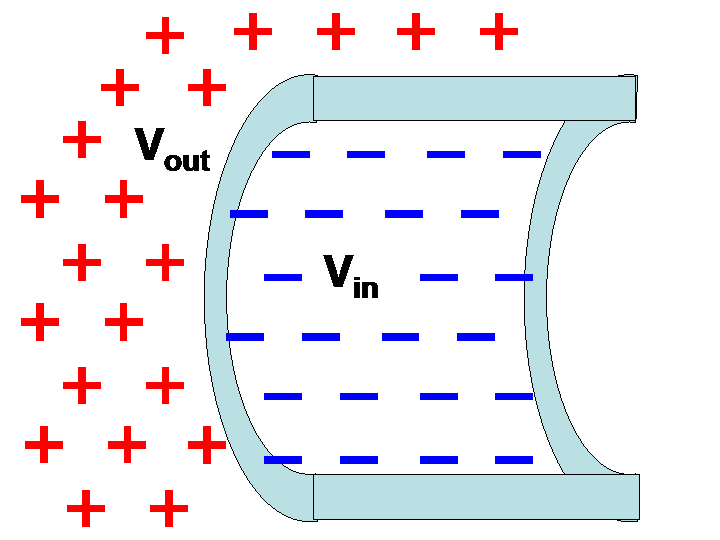
\includegraphics[width=3.0in]{./figures/Topic8/Fig8-2.png}
	\caption{A membrane with outside potential $V_1$ and inside potential $V_2$.}
 	\label{Fig8-2}
\end{figure}
The overall potential is calculated by taking into account the collective influence of all ions, which are the positively or negatively charged particles on either side of the membrane.  Each ion has a certain charge, $q$, which must be an integer number of electron charges ($q = \pm 1e^-, \pm 2e^-, \pm 3e^-, \cdots$).  Ion charges are quantified in Coulombs (C).  The charge of the electron, $e^-$, is $-1.6\times10^{-19}$ C.    
For a given potential $V$, an ion will have an electric potential energy $E$ given by
\begin{equation}
\label{eqn8-3}
E=qV.
\end{equation}
Thus, the potential energy of an ion $q$ depends on which side of the membrane it is on.  Ions on the outside have a potential energy equal to $E_{out} = qV_{out}$, and ions on the inside have a potential energy equal to $E_{in} = qV_{in}$.  Using the Boltzmann factor, we see that the relative probability of finding an ion on the outside of the membrane relative to the inside is
\begin{eqnarray}\label{eqn8-4}
\frac{P\left(E_{out}\right)}{P\left(E_{in}\right)}&=&\frac{{\rm e}^{-qV_{out}/k_BT}}{{\rm e}^{-qV_{out}/k_BT}}\nonumber\\
&=&{\rm e}^{-q\left(V_{out}-V_{in}\right)/k_BT}
\end{eqnarray}
The probability of finding an ion on a particular side of the membrane is directly proportional to the concentration of ions, $[C]$.  In mathematical terms, $$\frac{[C]_{out}}{[C]_{in}}=\frac{P\left(E_{out}\right)}{P\left(E_{in}\right)}.$$  By substitution, $$\frac{[C]_{out}}{[C]_{in}}={\rm e}^{-q\left(V_{out}-V_{in}\right)/k_BT}.$$  Solving for $V_{out}-V_{in}$, we arrive at the Nernst Equation, which is often used to calculate membrane potentials from ionic concentrations and vice-versa:
\begin{equation}\label{eqn8-5}
V_{out}-V_{in}=-\frac{k_BT}{q}\ln\left(\frac{[C]_{out}}{[C]_{in}}\right)
\end{equation} 
In physiology textbooks, the Nernst Equation is often written in terms of log base-10. $$2.3\log_{10}\left(\frac{[C]_{out}}{[C]_{in}}\right) = \ln\left(\frac{[C]_{out}}{[C]_{in}}\right)$$ If, for example, the charge $q$ of the ion is $\pm e^-$ ($\pm1.6\times10^{-19}$ C), and $T$ be the core temperature of the body, 310 K, we obtain the equations 
\begin{align}\label{eqn8-6}
V_{out}-V_{in}  &=  - 61~{\rm mV}\log_{10}\left(\frac{[C]_{out}}{[C]_{in}}\right)   & {\rm positive~ion}\\
V_{out}-V_{in}  &=  + 61~{\rm mV}\log_{10}\left(\frac{[C]_{out}}{[C]_{in}}\right)   & {\rm negative~ion}                         
\end{align}

Consider the concentrations (moles/m$^3$ or millimolar) for various ions outside and inside mammalian nerve cells, shown in Table \ref{table8-3}.
\begin{table}[htb]
\begin{center}
\begin{tabular}{|c|c|c|}
\hline
Ion & $[C]_{out}$ & $[C]_{in}$\\
\hline
K$^+$  &	5   & 140\\
Cl$^-$ &	110 & 4--30\\
Na$^+$ &	145 & 5--15\\
\hline
\end{tabular}
\caption{Ion concentrations outside and inside nerve cells.}
\label{table8-3}
\end{center}
\end{table}
Since potassium ions (K$^+$) are positive, we use Eq.~8.6:
$$V_{out}-V_{in}  =  -61~{\rm mV}\log_{10}\left(\frac{5}{140}\right)= +88~{\rm mV}.$$
Since chloride ions (Cl$^-$) are negative, we use Eq.~8.7:
$$V_{out}-V_{in}  =  +61~{\rm mV}\log_{10}\left(\frac{110}{4~{\rm to}~30}\right)= -34~{\rm to}~88~{\rm mV}.$$
These results agree reasonably with experiments that find the potential inside a nerve cell to be about 70 mV lower than the potential on the outside.  From this we conclude that K$^+$ ions and Cl$^-$ ions are in equilibrium with those potentials.  Let us now do the same calculation for sodium (Na$^+$) ions.  Since sodium ions are positive, we use Eq.~8.6 again:  
$$V_{out}-V_{in}  =  -61~{\rm mV}\log_{10}\left(\frac{145}{5~{\rm to}~15}\right)= -60~{\rm to}~-89~{\rm mV}.$$
The negative result implies that sodium ions are not in equilibrium, so there must be some non-equilibrium process going on to drive the ions up the concentration gradient.  This effect is achieved by the well-established sodium-potassium pump model.  The pump requires energy in the form of ATP to move three sodium ions out of the cell for every two potassium ions that enter the cell.  The pump will be discussed again in Topic 11 on nerve conduction, when we shall see that maintenance of the voltage difference across the cell membrane is critical to neuron function.

\subsection{Protein Folding and Structure Prediction: Background}

Proteins are naturally occurring polymers that play many fundamental roles in a cell.  They are classified into three groups according to their shape and function:
\begin{itemize}
\item Fibrous proteins contribute to the composition of bones, hair, feathers, tendons, and skin.
\item Membrane proteins are responsible for the transport of substances across the cell membrane.
\item Globular proteins facilitate specific chemical reactions within the cell.
\end{itemize}	
By understanding protein structure from physical principles, and by allowing computers to rapidly model protein folding under a variety of conditions difficult to study in the laboratory, we can gain new insight into drugs and diseases that function at the molecular level.  Alzheimer’s disease, cystic fibrosis, mad cow disease, a number of cancers, and many other diseases are caused by misfolded proteins.

All proteins are made up of monomers called amino acids.  Some of the amino acids, called nonessential amino acids, are synthesized naturally by the body.  Others are called essential amino acids, because they must be ingested in the diet.  There are 20 naturally-occurring amino acids found in proteins.  
The sequence of amino acids in any protein is unique -- it is this sequence, or primary structure, that determines the protein's secondary structure (alpha helix and beta sheet) which determine the protein's overall shape (tertiary structure) and thus its function in the cell.  Scientists can somewhat easily isolate a protein and determine its primary structure.  It is much more difficult to discover its three-dimensional tertiary structure, though methods like x-ray crystallography and nuclear magnetic resonance are routinely used for this purpose (see Topic 9).  Because these techniques are so labor- and time-intensive, we would rather be able to accurately predict the 3D structure of a protein just by knowing its primary structure.

As we shall see, this task is surprisingly difficult.  Before we try to tackle structure prediction, we must first understand how proteins are produced in the body.  The genetic material of the cell, called deoxyribonucleic acid (DNA), governs when and how much of a protein will be synthesized.  Just as proteins are polymers of 20 different monomers called amino acids, DNA molecules are polymers of four different monomers called bases: adenine (A), guanine (G), thymine (T), and cytosine (C).

We can think of DNA as an information storage device like a computer.  A computer stores digital information in its sequence of bits, and DNA stores information about proteins in its sequence of bases.  For computers, the bit is the fundamental unit of information, assuming one of two values: on or off (1 or 0).  Bits are grouped into words, each of which codes for a number, a text character, or an instruction to the processor.  A computer program is nothing more than a long sequence of these words.  Complex programs are organized into a collection of smaller programs known as subroutines, each of which performs a single task within the program.  Similarly, the base is the fundamental unit of information for DNA, assuming one of four values: A, G, T, or C.  Bases are grouped into three-letter sequences called codons (analogous to words), each of which codes for a specific amino acid.  The order of codons in a segment of DNA determines the order of amino acids in the protein, just as the order of words in a computer program determines, for example, the order of text characters to be displayed on the screen.  If we think of the entire genetic code of the cell, called the genome, as a complex computer program, genes are analogous to subroutines: each is called upon to instruct the synthesis of a specific protein.

Humans have about 30,000 genes altogether, which are turned on and off by elaborate cascades of protein interactions.  When the cell needs a certain protein to be manufactured, two steps must occur.  The first step, called transcription, takes place when a single-stranded DNA-like molecule called messenger RNA (mRNA) copies the segment of DNA corresponding to a protein and brings it out of the nucleus.  When it reaches an organelle called the ribosome, the second step of protein synthesis, called translation, takes place.  Specialized molecules, known as transfer RNA (tRNA) molecules, recognize the codons and allow the appropriate amino acids to polymerize in a linear fashion to form the protein.

As mentioned before, there are twenty different amino acids ubiquitous in all life forms.  Figure \ref{Fig8-3} gives the structure and three-letter abbreviation for each.\footnote[4]{Courtesy of \href{http://www.biochem.ucl.ac.uk/bsm/dbbrowser/c32/aastruct.html}{http://www.biochem.ucl.ac.uk/bsm/dbbrowser/c32/aastruct.html}.}
 \begin{figure}[!h]
 	\centering
 	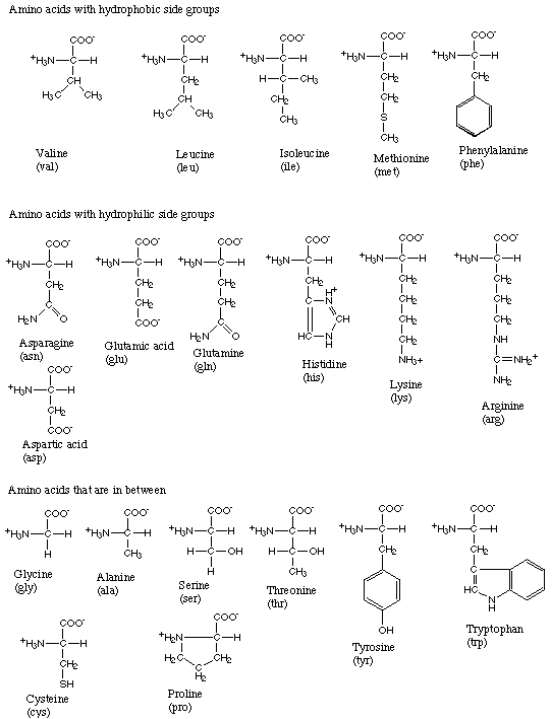
\includegraphics[width=\textwidth]{./figures/Topic8/Fig8-3.png}
 	\caption{The amino acids.}
  	\label{Fig8-3}
 \end{figure}

As you can see, each amino acid consists of a carbon atom that binds four chemical groups: an amino group (NH$_3^+$), a carboxyl group (COO$^-$), a hydrogen atom (H), and a unique group commonly denoted by ``R''. The R group is usually referred to as a ``side chain'' since it protrudes off the axis of the protein, as shown in Figure \ref{Fig8-4}.   
\begin{figure}[htb]
 	\centering
 	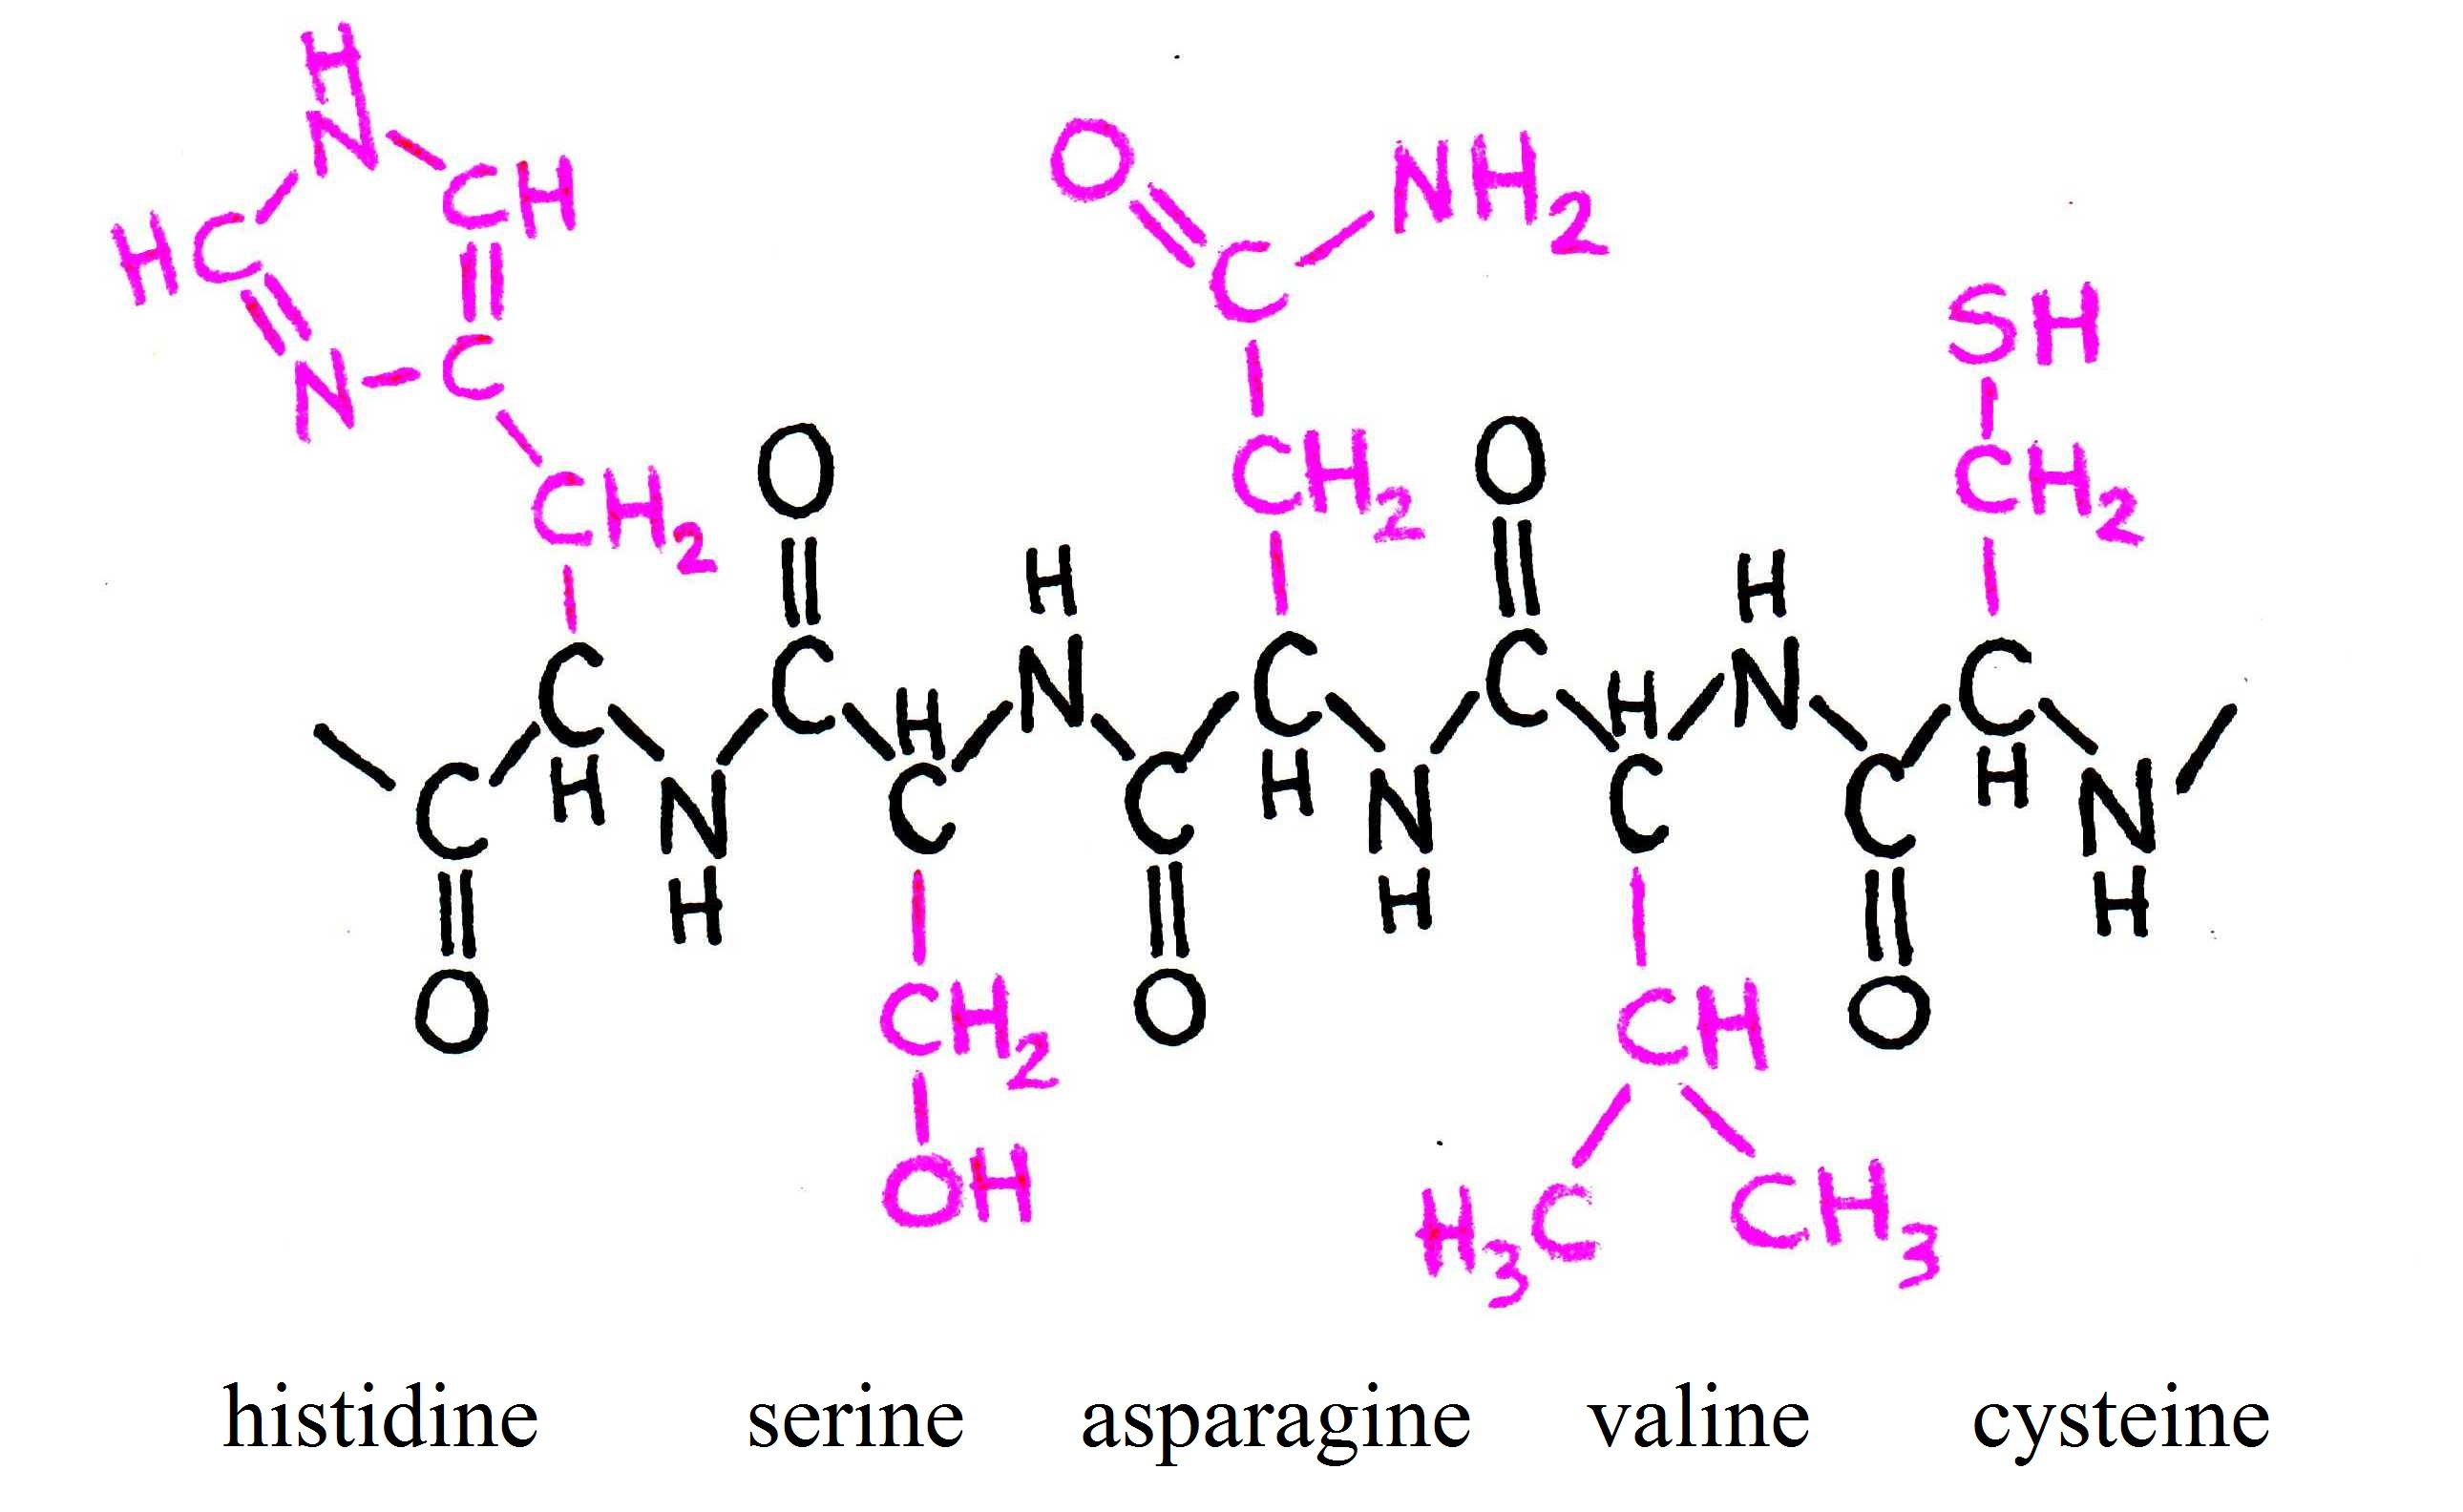
\includegraphics[width=\textwidth]{./figures/Topic8/Fig8-4.jpg}
 	\caption{Five amino acids bound together.  Notice that the R groups protrude from the plane of the amino acid.}
  	\label{Fig8-4}
\end{figure}

Side chains differentiate amino acids from one other and determine how they interact with their environment.  Some of the side chains are polar, meaning they contain regions of separated or partially separated electric charges.  Because ``like dissolves like,'' these polar side chains interact favorably with polar solvent molecules like water and are thus called {\it hydrophilic} side chains.  Other side chains are nonpolar and only mix well with nonpolar molecules, like the lipids that make up cell membranes.  These side chains are termed {\it hydrophobic}.  Still other amino acids fall between these two extremes.  The side chains thus play a key role in controlling how each protein site is attracted or repelled by its environment, and ultimately how the protein folds to achieve its biological function.  For example, hydrophobic amino acids tend to cluster in the center of a globular protein to avoid contact with water, while hydrophilic amino acids tend to cover the surface of the protein that is in contact with the aqueous environment.  Similar effects take place around so-called transmembrane proteins, which are partially embedded within a membrane.  The portion of the protein embedded in the membrane is hydrophobic, while the amino acids exposed to the cytosol and extracellular fluid are primarily hydrophilic.  Returning to Figure \ref{Fig8-2}, we see how amino acids can be grouped according to the hydrophobicity of their side chains.
     
Both a protein's environment and its unique order of amino acids determine how it assumes its specific three-dimensional fold.  Within milliseconds of formation, the protein assumes this 3D structure.  Under physiological conditions (pH $\sim$7.0; $T$ = 310 K), the protein's geometry, known as the native state, is marginally stable (40 kJ/mole or 0.4 eV/molecule).  Under non-physiological conditions, the protein can unfold into a variety of conformations.  When this happens, it is said to denature.  The transition between native and denatured states is very sudden -- at some temperature or pH change, the protein undergoes a sudden phase transition.  This transition is often reversible by the appropriate change in the environment.
  
Since the structure of a protein (and thus its function) is encoded in its amino acid sequence, one might think that there must be a ``code'' that translates the sequence into a 3D conformation.  Unfortunately, this code has proved extremely difficult to crack due to its complexity.  To predict the shape of the protein from the amino acid sequence, a number of effects must be taken into account.  These include the bond forces and torques between adjacent amino acid and the possibility of hydrogen, ionic, and covalent bonding between distant amino acids.  Furthermore, external factors like temperature, pH, and solvation must be considered.

\subsection{Protein Structure Prediction and the Boltzmann Factor}

As mentioned before, predicting protein structures from amino acid sequences is an arduous task, even with today’s computer technology.  So how do we begin to do it?  We assume that a protein folds to assume the lowest possible energy state and then use the connection between energy and probability -- the Boltzmann factor -- to develop computer algorithms for prediction.    

Let us now look more closely at the fundamental principles that drive protein formation.  When two amino acids join to form a protein, a bond forms between the carboxyl group of one and the amino group of the other.    
\begin{figure}[htb]
 	\centering
 	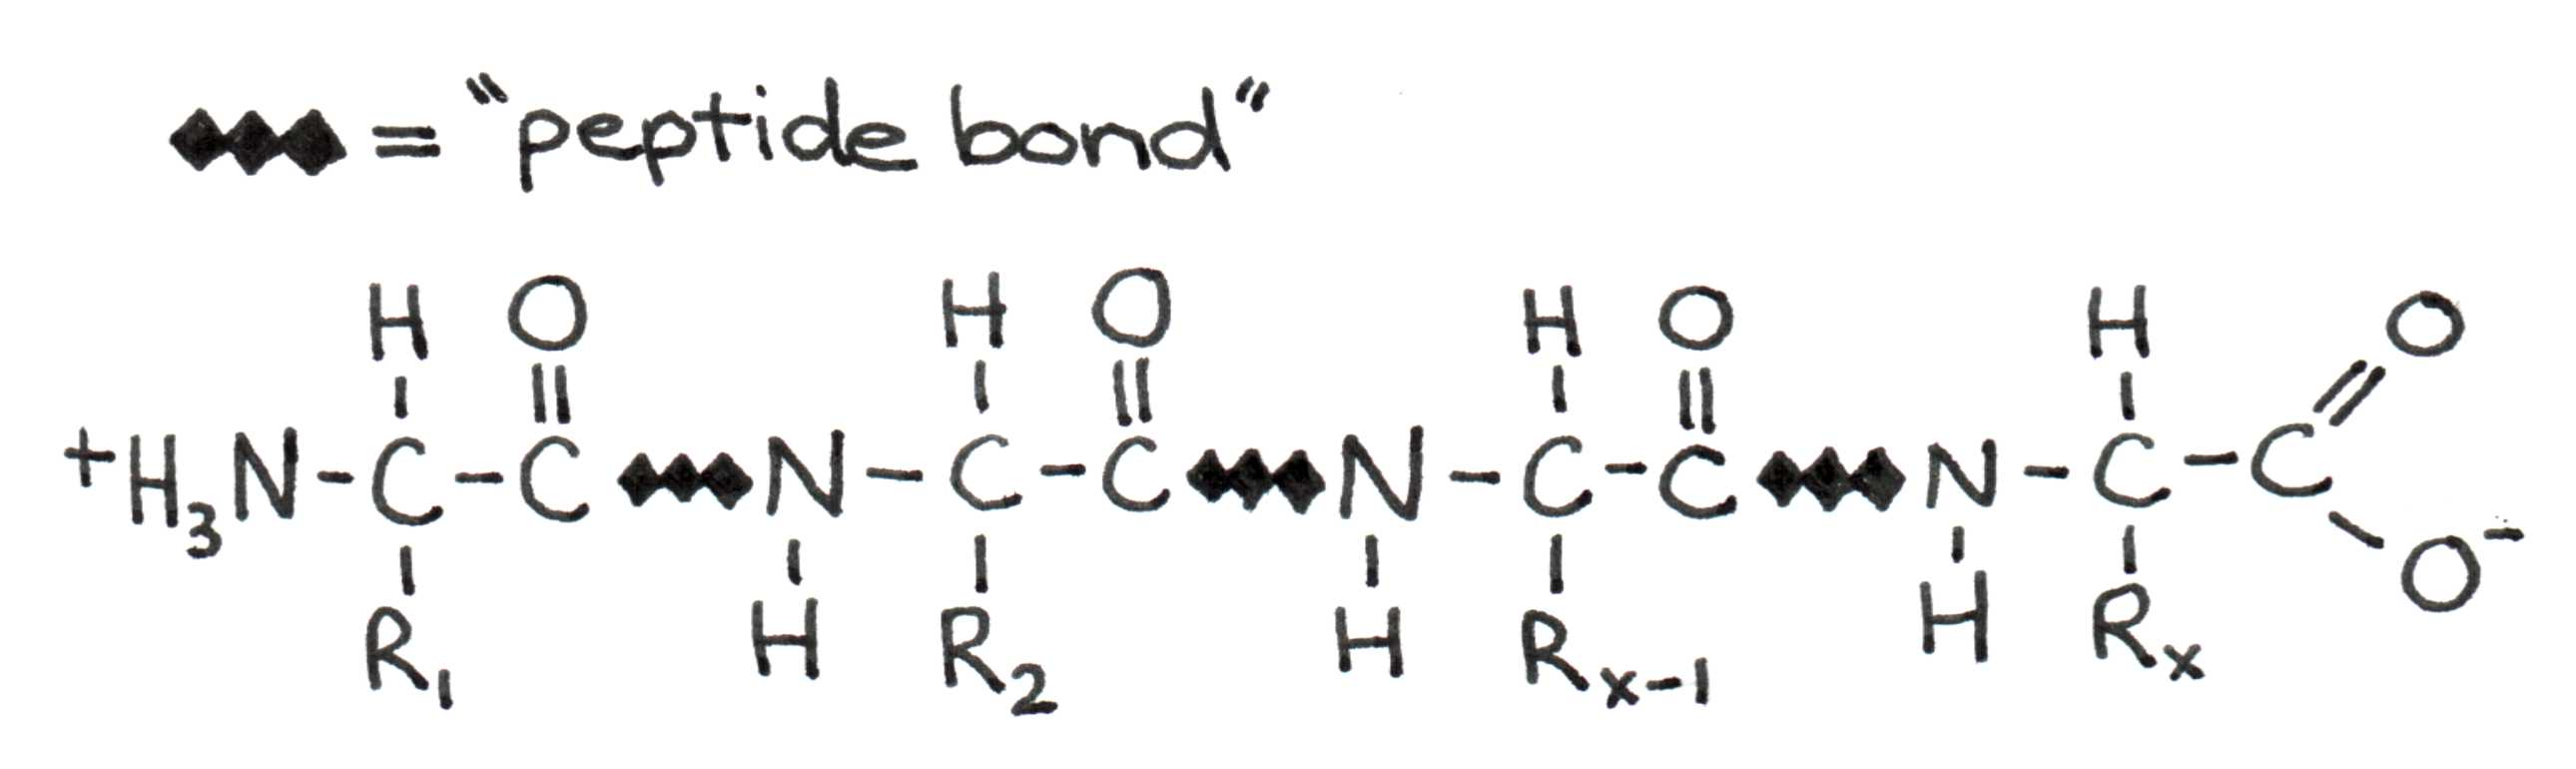
\includegraphics[width=\textwidth]{./figures/Topic8/Fig8-5.jpg}
 	\caption{Four amino acids linked in a polypeptide chain.  The C-N bond between amino acids is called the peptide bond.}
  	\label{Fig8-5}
\end{figure}

To fully understand how a protein folds, we must first examine how a pair of adjacent amino acids can twist relative to one another.  The bonded carboxyl (C=O) and amino (N-H) groups form a rigid planar unit called the peptide group.  The molecule cannot twist about the C-N bond, but the central alpha carbon (C$_{\alpha}$) can act as a pivot point for the C$_{\alpha}$-C and C$_{\alpha}$-N bonds, as shown in Figure \ref{Fig8-6}.
\begin{figure}[htb]
 	\centering
 	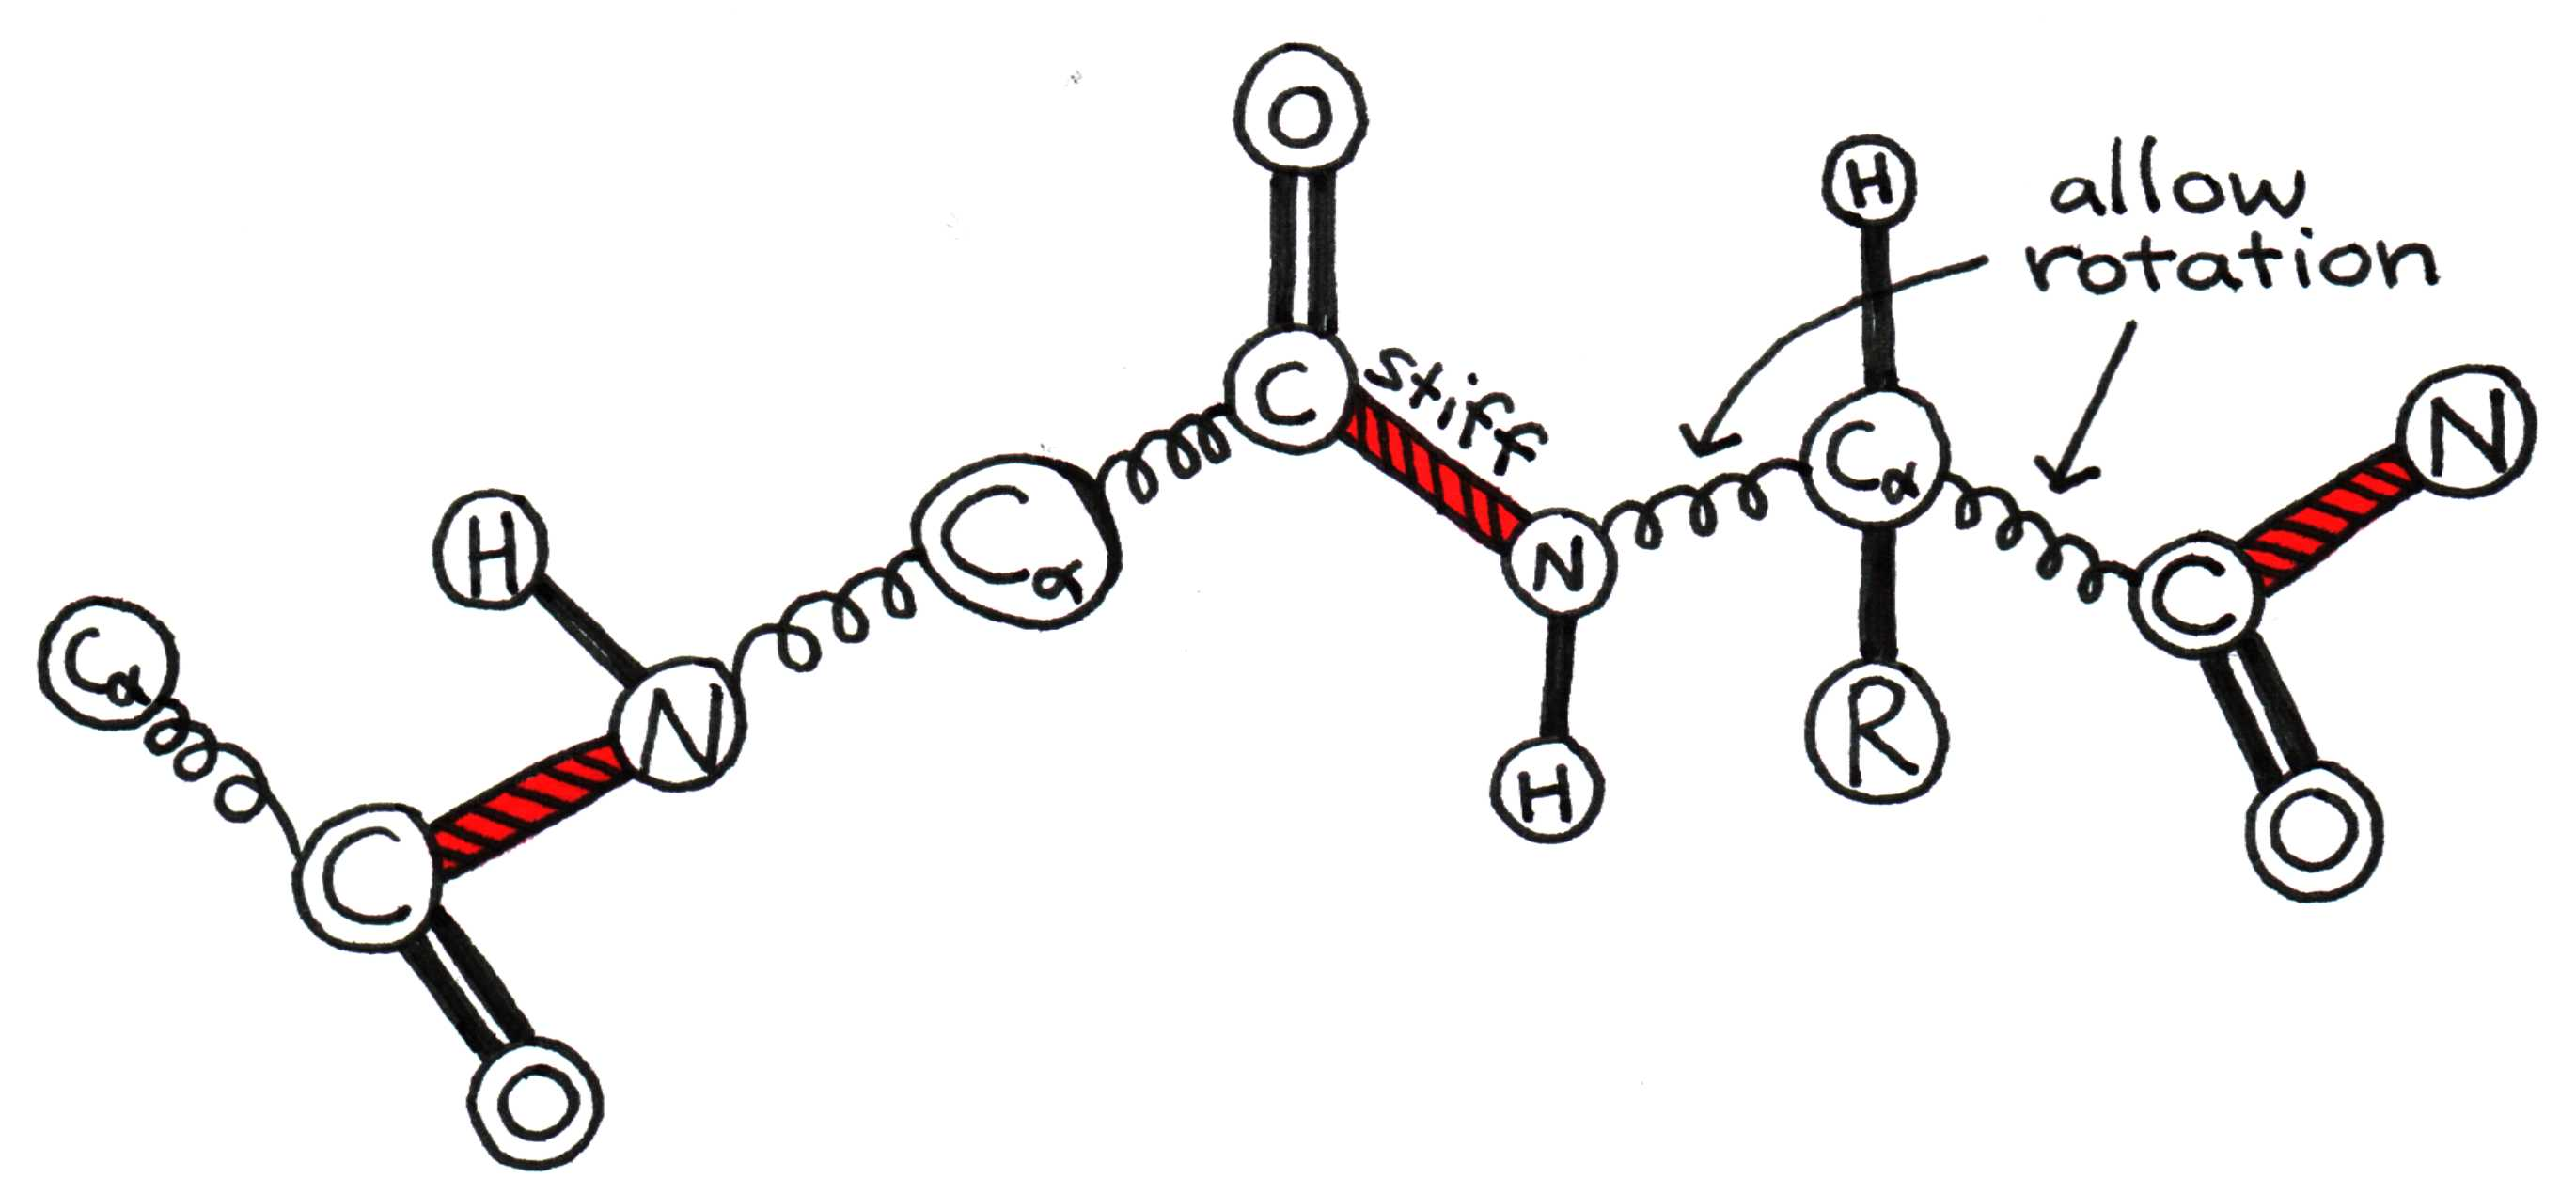
\includegraphics[width=\textwidth]{./figures/Topic8/Fig8-6.jpg}
 	\caption{The alpha carbon acts as a pivot around which peptide groups can rotate.}
  	\label{Fig8-6}
\end{figure} 
To obtain an appreciation for the problem of modeling, assume for simplicity that each peptide group can have one of four orientations relative to adjacent groups.  In other words, the angle $\theta$ between peptide groups can have one of four values.  For a protein with 100 amino acids, this yields an astounding $4^{99} = 4\times10^{59}$ possible angle arrangements, or protein conformations.  A long-standing mystery in biology is how nature determines the correct conformation out of all these possible combinations -- within nano to milliseconds of formation.  We do not yet fully understand how protein folding occurs so quickly, but we do know that the protein arrives at the conformation with the lowest potential energy.  Thus, to predict shape, we must take up the tools of statistical mechanics, as discussed earlier in this chapter.  From a statistical perspective, the correct conformation should be the most probable one.  Consider a protein of $n$ amino acids.  Letting $\theta_1$ be the angle between the first two amino acids, the probability of the bond having torsional energy $E(\theta_1)$ is related to the Boltzmann factor, $P_1\propto{\rm e}^{-E\left(\theta_1\right)/k_BT}$.  Similarly, if $\theta_2$ is the angle between the second and third amino acids, the probability of the bond having torsional energy $E(\theta_2)$ is $P_2\propto{\rm e}^{-E\left(\theta_2\right)/k_BT}$.  The pattern continues in the same way for the rest of the angles.  If we wish to know the probability of the protein having a specific conformation (a specific set of orientations $\theta_1, \theta_2, \theta_3,\cdots, \theta_{n-1}$) we simply multiply all the individual probabilities together:
\begin{eqnarray}\label{eqn8-8}
P_{total} &=& P_1 \cdot P_2 \cdot P_3 \cdots P_{n-1}\nonumber\\
&=& C{\rm e}^{-E\left(\theta_1\right)/k_BT}\cdot{\rm e}^{-E\left(\theta_2\right)/k_BT}\cdot{\rm e}^{-E\left(\theta_3\right)/k_BT}\cdots{\rm e}^{-E\left(\theta_{n-1}\right)/k_BT}\nonumber\\
&=& {\rm e}^{-\left(E\left(\theta_1\right)+E\left(\theta_2\right)+E\left(\theta_3\right)+\cdots E\left(\theta_{n-1}\right)\right)/k_BT}
\end{eqnarray}
When the sum of all the energies in Eq.~\ref{eqn8-8} is minimized, the overall probability is maximized.  Computer programs can evaluate the lowest energy conformation by assuming that molecular bonds can be modeled as classical elastic forces, while the interactions between amino acids and water or other molecules can be modeled as classical electrostatic forces.  Thus, each angle orientation has a certain combination of mechanical and electrical energy associated with it.

Energy minimization routines begin by calculating the total energy $E(\theta_1) + E(\theta_2) + \cdots + E(\theta_{n-1})$ of a certain conformation.  Then the angles are changed slightly and the sum reevaluated.  If the energy is lower, the program continues to change the angles in that direction.  These steps are repeated until a minimum energy is found.  The method is useful, but it does not guarantee that the absolute minimum will be found, since the algorithm stops as soon as any minimum -- global or local -- is found. There are routines for attempting to determine whether a minimum is global or local, but they do not always work.  
\begin{figure}[htb]
 	\centering
 	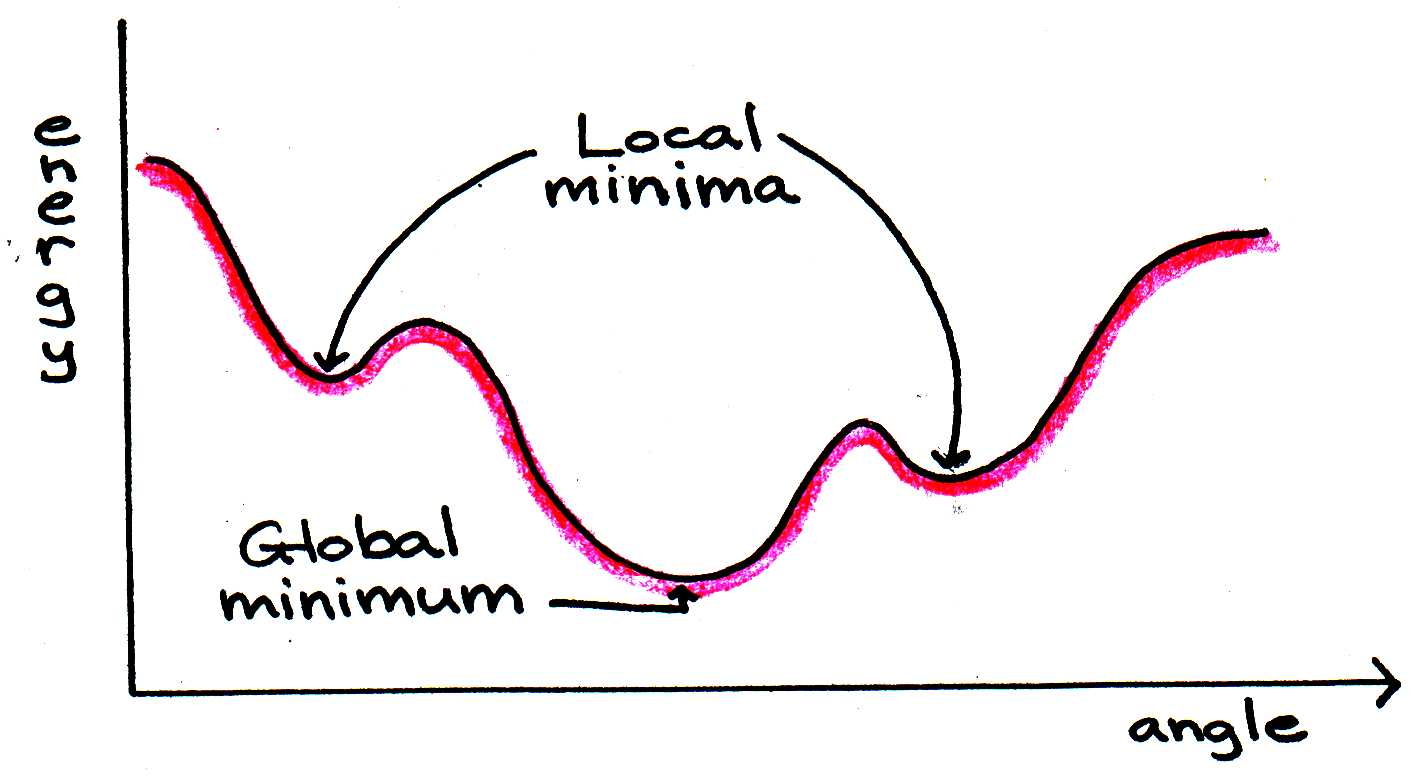
\includegraphics[width=\textwidth]{./figures/Topic8/Fig8-7.jpg}
 	\caption{Energy minimization programs do not always arrive at the global minimum if the starting sum is closer to a local minimum.}
  	\label{Fig8-7}
\end{figure}
To verify that the global minimum has really been found, the computer program can ``heat'' the protein to alter its conformation slightly and then cool it slowly, allowing the protein to reassume its fold.  By disturbing the protein's structure in this way, we seek to release it from a local energy minimum ``trap.''  The algorithm then continues as before until the energy changes become negligible.